% Text that has been removed from the draft.

Significant cross-link anisotropy is expected mainly for enzymatic cross-links created during fibril formation. For fibrils with significant post-formation cross-linking due to advanced glycation end-products (AGEs), we might expect a decrease in the effective anisotropy $\zeta\to1$ as the ratio of AGE-induced to enzymatic cross-links increases. Nonetheless as long as there is some degree of anisotropy, $\zeta$ will remain strictly greater than $1$. Other structural changes such as mineralization may also impact the cross-link anisotropy in as-yet unknown ways. Altering $\zeta$ experimentally may be a possible avenue through which to tune mechanical properties of lab-grown fibrils.


%Human, bovine and rat tendon fibrils have an extensibility before failure of between $20$ and $30\%$ \cite{Quigley:2018, Svensson:2013}. This is similar to the largest D-band strains  -- $20\%$ -- observed for bovine and rat tendon fibrils stretched on an elastic substrate \cite{Gachon:2020, Peacock:2019}. In order to achieve such large strains without losing the molecular density fluctuation responsible for the D-band spacing, tendon fibrils must deform by a combination of molecular sliding \cite{Gautieri:2017, Peacock:2019} and/or molecular stretching \cite{Iqbal:2019} -- mechanisms that we have not modelled here. 

%Indeed, based on geometrical considerations, deformation via molecular untwisting can only accommodate strains up to  $\epsilon_\mathrm{untwist}^\mathrm{max}=\sec\left[\psi_0(R)\right]-1$. While this limit can be as high as $5-6\%$ strain in highly twisted corneal tissue, it is less than half a percent for the small molecular twist of tendon fibrils. We thus expect that the torsion-stretch coupling described here is negligible in tendon, and D-band strain should be a good measure of fibril strain. 

%However, the strains at failure are much larger than can be recovered with our model -- indicating that other mechanisms are at play in fibril strain such as molecular sliding \cite{Gautieri:2017, Peacock:2019} or stretching \cite{Iqbal:2019}.

This condition is easily satisfied for the parameters we estimate for corneal fibrils in section \ref{cornealcompare}. In cases when the condition on $\zeta$ and $\langle\psi_0^2\rangle$ is not satisfied, the D-band strain can instead overestimate the fibril strain for small $\epsilon_F$. Due to the concavity of eq.~\ref{DbandvsFibril} however, we will always recover $\epsilon_D<\epsilon_F$ at larger fibril strains.

%%%%%%%%%%%%%%%%%%%%%%%%%%%%%%%%%%%%%%%%%%%%%%
\begin{table}[htb]
\centering
\begin{tabular}{|c l l|} 
\hline
 $\psi(r)$ & Twist angle function & \\ 
 $r$ & Radial coordinate &  \\
 $d$ & D-band spacing & \\
 $\zeta$ & Cross-link anisotropy  &\\
 $\epsilon_D$ & Axial D-band strain & \\
  $\epsilon_F$ & Axial fibril strain & \\
 \hline
\end{tabular}
\caption{Key variables and parameters.}
\label{table:paramtable}
\end{table}

%\subsection{Non-small angle}  
% ML: If we do decide to include this, here are some things we could say:

% lambda->infity limit
% In this limit we have $\epsilon_D = \left( \frac{\langle \cos^2\psi_0\rangle}{\langle\cos^4\psi_0\rangle}\right)^{1/2} - 1$.
% we already mention this in the previous subsection

% zeta -> 1
% In this limit we have:
%\begin{equation}
%\epsilon_D = \begin{cases} 
%0, & \epsilon_F=0\\
%\left( \frac{\langle \cos^2\psi_0\rangle}{\langle\cos^4\psi_0\rangle}\right)^{1/2} - 1, & \epsilon_F>0.
%\end{cases}
%\end{equation}

% zeta -> infity
% Don't think I can say anything about this limit for large psi.

% ADR: attribute monotonicity to earlier paper (of psi)
% ML: In general psi is a monotonically decreasing function of epsilon_F as long as zeta>1. (pretty straightforward to show by checking the derivative)

% Anecdotally (based on numerical investigation) we always find $\partial \epsilon_D/\partial\epsilon_F \geq0$ and $\partial^2 \epsilon_D/\partial\epsilon_F^2 \leq0$ (D-band strain is a monotonically increasing and concave function of fibril strain) as long as zeta>1 and epsilon_F>0.
% We already say this in the preceding section.


%%%%%%%%%%%%%%%%%%%%%%%%%%%%%%%%%%%%%%%
% CUTOUTS:

%strain is applied to the fibril, additional free energy contributions need to be considered to account for the energy cost of deforming the intermolecular cross-links. We use a free energy term derived from the neoclassical theory of rubber elasticity, which models cross-link deformation under strain in nematic liquid crystals \cite{Warner:1996}. The scale of this energetic contribution, on the same order as the fibril's elastic sheer modulus, dominates the terms from the Frank and D-band free energies by several orders of magnitude \cite{Leighton:2021}. As such, the deformation of the molecular director field will be determined entirely by minimization of the elastomeric free energy term. This minimization can be performed analytically \cite{Leighton:2021b}, and yields an expression for the twist angle function $\psi(r)$ as a function of the initial twist function $\psi_0(r)$ and the fibril stretch ratio $\lambda$:

In Fig.~\ref{fig:dbandvsfibrilstrain} we show D-band strain $\epsilon_D$ as a function of fibril strain $\epsilon_F$ for several different initial twist functions. In particular, we consider a constant $\psi_0(r) = 0.1$ radians ($\approx 5^\circ$), a linear $\psi_0(r) = 0.3 r/R$ similar to previous predictions for corneal fibrils, and a concave $\psi_0(r) = 0.3\tanh(2r/R)$ which is very similar to the general class of twist angle functions predicted by coarse-grained modelling of cross-linked fibril growth \cite{Leighton:2021}. We also show in \ref{fig:dbandvsfibrilstrain}D a convex twist function, $\psi_0(r) = 0.3 \left(r/R\right)^8$, which satisfies both $\langle\psi_0^2\rangle=0.01\text{rad}^2$ and $\psi_0(R)=0.3\text{rad}$, and may better reflect the corneal fibrils experimented on in \cite{Bell:2018}.

\begin{figure}[h] 
\centering
  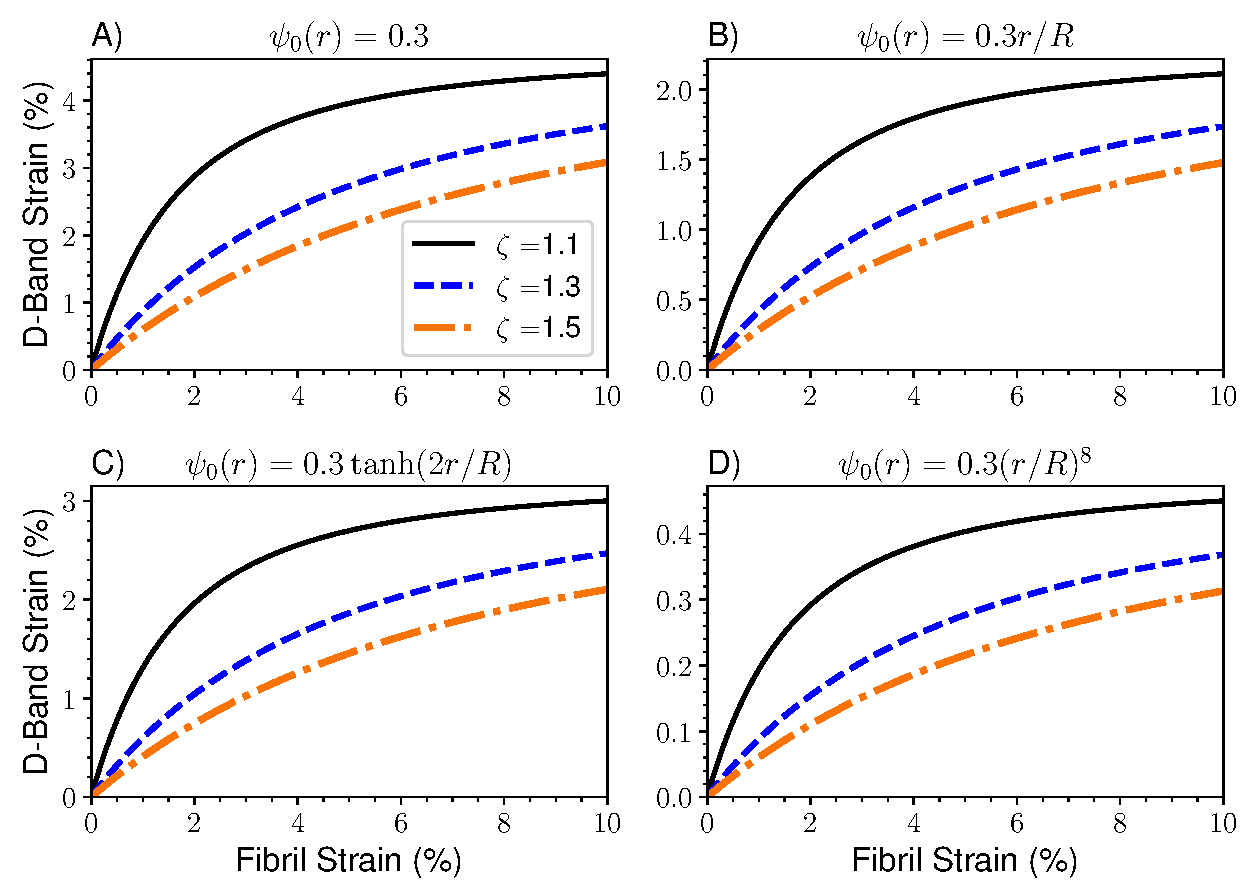
\includegraphics[width=14cm]{Figure_2.pdf}
  \caption{We plot D-band strain vs Fibril strain several different unstrained twist-angle functions: A) a constant twist, B) a linear twist, C) a concave twist function, and D) a convex twist function that satisfies both $\langle\psi_0^2\rangle=0.01\text{rad}^2$ and $\psi_0(R)=0.3\text{rad}$.}
  \label{fig:dbandvsfibrilstrain}
\end{figure}

%Instead, we can minimize $f_D$With one value of $d$ for the D-band, $d_\parallel$ cannot be satisfied everywhere within the fibril due to the molecular twist-field. Instead local sliding or stretching of collagen molecules occur to adjust the local D-band, as well as a global accommodation of the D-band period. 


% Add a short section on the potential for reversibility of the molecular tilt.

%In the cornea, Collagen fibrils have a molecular tilt at the surface between 16 and 24 degrees. For such highly tilted fibrils there is a regime before molecules are stretched where any applied fibril strain induces a sharp decrease in molecular tilt and a small D-band strain. In this case the fibril strain can be obtained by fitting the molecular tilt versus D-band strain trend. We also extract the average molecular tilt squared of the fibrils before deformation which provides new structural information about the fibrils (Fig.~\ref{fig:dbandstrain}).

%Combining this estimate with the known surface twist of corneal fibrils, generally around $0.28-0.31$ radians ($\approx 16-18^\circ$), suggests that corneal collagen fibrils may exhibit convex twist angle functions. Here we use the term ``convex" to denote a positive second derivative $\psi''(r)>0$.

%In order to achieve such large strains without losing the molecular density fluctuation responsible for the D-band spacing, tendon fibrils must deform by a combination of molecular sliding \cite{Gautieri:2017, Peacock:2019} and/or molecular stretching \cite{Iqbal:2019}. 






%%%%%%%%%%%%%%%% Alternate strain discussion:

Based on geometrical considerations, the maximum strain that can be accommodated by the deformation mechanism we have described--molecular untwisting is on the order of
\begin{equation}\label{max_untwist_strain}
\epsilon_\mathrm{untwist}^\mathrm{max}\approx \sec\left[\psi_0(R)\right] -1.
\end{equation}
For fibril strains significantly larger than $\epsilon_\mathrm{untwist}^\mathrm{max}$ other modes of deformation, such as stretching or sliding of molecules, must come into play. In this regime D-band strains could become much larger than the upper bound we have predicted ($\epsilon_D^\mathrm{max} \simeq \langle\psi_0^2\rangle/2$) based on molecular untwisting alone.

When the surface molecular twist is smaller than $5^\circ$, as in tendon fibrils \cite{Hulmes:1981}, strain-straightening of molecules is not a significant deformation mechanism. Indeed, from equation \ref{max_untwist_strain}, deformation via molecular untwisting in tendon should only be significant for fibril strains less than about half a percent. We thus expect that the torsion-stretch coupling described here is negligible and D-band strain should be a good measure of fibril strain. Human, bovine and rat tendon fibrils have an extensibility before failure of between $20$ and $30\%$ \cite{Quigley:2018, Svensson:2013}. This is similar to the largest D-band strains  -- $20\%$ -- observed for bovine and rat tendon fibrils stretched on an elastic substrate \cite{Gachon:2020, Peacock:2019}. In order to achieve such large strains without losing the molecular density fluctuation responsible for the D-band spacing, tendon fibrils must deform by a combination of molecular sliding \cite{Gautieri:2017, Peacock:2019} and/or molecular stretching \cite{Iqbal:2019}, phenomena which we have not modelled here. 